\documentclass[11pt,a4paper]{article}

\usepackage[T1]{fontenc}
\usepackage[utf8]{inputenc}
\usepackage{lmodern}
\usepackage[margin=2.4cm]{geometry}
\usepackage{amsmath,amssymb,bm}
\usepackage{booktabs,array,tabularx,multirow}
\usepackage{graphicx}
\usepackage{enumitem}
\usepackage{xcolor}
\usepackage{tikz}
\usetikzlibrary{arrows.meta,decorations.pathreplacing,calc,patterns,positioning}
\usepackage[colorlinks=true,linkcolor=teal!70!black,citecolor=teal!70!black,urlcolor=teal!70!black]{hyperref}
\usepackage{caption}
\captionsetup{font=small,labelfont=bf}

\setlength{\parskip}{0.4em}
\setlength{\parindent}{0pt}
\newcommand{\nj}{\textsc{nj}}
\newcommand{\nh}{\textsc{nh}}
\newcommand{\tcross}{\tau_{\mathrm{cross}}}

\title{\textbf{Scheduling a Shared Mobile Head Across Parallel Conveyors with Endogenous Blocking}\\[0.3em]
\large A sampled-future look-ahead and the learned dispatching policy that amortizes it}
\author{laser-conveyor-optimization\\\small\url{https://github.com/juanlopez-gif/laser-conveyor-optimization}}
\date{November 2026 --- draft 0.1 (results of versions 0.7.5--0.7.13)}

\begin{document}
\maketitle

\begin{abstract}
A single XY laser head serves parts that arrive on several parallel conveyors. A part can
be processed only inside a working zone; while it is processed its conveyor stops, and an
unprocessed part that reaches the end of the zone stops its conveyor until the head serves
it. The availability of every part therefore depends on the schedule itself (endogenous
blocking), the parts keep arriving during the operation, and the controller sees only what
is on the belts. We formulate the problem, show that it is strongly NP-hard with the number
of conveyors in the input, and ask how to decide well in milliseconds. The method has two
parts. A look-ahead search scores each candidate part by simulating the known parts
together with sampled futures of the unknown arrivals (eight Poisson futures over a 30~s
window, common random numbers, the realized cost of every part as the objective); it is
the best decision rule we found, but it needs about a second per decision. A
permutation-invariant Transformer policy over the parts, the belts, the head and the cell's
parameters, trained by expert iteration on randomized cells with one to six conveyors,
amortizes that search: on 30 reserved realizations of eight operating regimes, used once,
the policy alone equals its teacher in every regime (within $\pm0.8$ points, never
significantly worse), beats the look-ahead over the known parts in every regime by
1.5--3.9 points (significant in seven), and beats the nearest-part rule by 2--7\,\% of the
penalized flow time in seven of the eight regimes, at 10.8~ms per decision (median, one
thread, machine fully loaded; 17.5~ms at the 95th percentile) against 1.2~s for the
search. Three negative results shape the method: truncating the look-ahead with a learned
value is far worse than not truncating; sampled futures help only when the look-ahead
counts every part, not only the known ones; and larger networks (6.7~M and 39~M
parameters) do not raise the ceiling set by the teacher. Giving the teacher the cell's
bursty arrival model does not improve it either. The distance to the optimum is not
measured and is the main open question.
\end{abstract}

%====================================================================
\section{Introduction}
%====================================================================
Cells in which one shared actuator serves several moving streams are common in sorting,
packaging and marking lines \cite{S01_Mattone2000,S02_Han2020,S03_Nielsen2023,S04_Schettini2023}.
In most of them the belt never stops for the actuator: an item that is not picked in time
leaves the window and is lost, and the scheduling problem is an interception problem with
fixed availability windows. The cell studied here is different in a way that changes the
problem's structure. A laser head marks parts on three parallel conveyors; marking a part
stops its conveyor for the processing time, and a part that reaches the end of the laser
zone unmarked stops its conveyor until the head serves it. Every decision therefore moves
the availability windows of the other parts on the same belt, and a late decision creates
blocking that propagates. Parts keep arriving while the cell runs, at rates the
controller knows but at instants it does not, and the controller observes only the parts
on the belts.

This paper asks how to decide well, fast, in that setting. Its contributions are:
\begin{enumerate}[nosep]
\item A formulation of the online problem with endogenous blocking and a partial
  information model (Section~\ref{sec:problem}), with its complexity (strongly NP-hard
  with the number of conveyors in the input) and the structural facts that matter for
  dispatching: belt order is not dominant, the first part of a conveyor is not always the
  one to serve, and a look-ahead over the known parts alone has a ceiling.
\item A look-ahead search for the online problem (Section~\ref{sec:search}) that
  simulates every candidate against sampled futures of the unknown arrivals and scores it
  by the realized cost of all parts. We report which design choices matter: the
  objective (all parts, not the known ones), the number of futures (eight), the window
  (20--30~s), and the failure of value-based truncation.
\item A learned dispatching policy (Section~\ref{sec:policy}) that reads the state as a
  set of tokens (parts, conveyors, head, cell parameters), points to any candidate part,
  and is trained by expert iteration on a distribution of cells with one to six
  conveyors. The policy reaches its teacher's quality and decides in 10~ms.
\item A pre-registered confirmatory evaluation on reserved realizations
  (Section~\ref{sec:confirm}): the policy against the nearest-part rule, the known-parts
  look-ahead and its own teacher, on eight regimes, with per-decision latencies, in the
  two action modes of the cell.
\end{enumerate}
A companion paper (Paper~2) uses the policy and the rule as controllers to measure the
value of upstream visibility and of pre-positioning; this paper is about the decision
method and uses the design mode of the cell only as a second action setting.

%====================================================================
\section{Related work}\label{sec:related}
%====================================================================
\textbf{Picking and sorting from moving conveyors.} With one arm over one belt and
Poisson arrivals, \cite{S02_Han2020} sequence the reachable objects by dynamic
programming and show that greedy rules (first-in, nearest-first) are not optimal in
general; the belt never stops and objects that leave the window are lost. Sorting on a
moving belt \cite{S01_Mattone2000} and value-aware sorting with availability windows
\cite{S05_Kokkalis2026} share that setting. With several arms, \cite{S03_Nielsen2023}
batch items from an infeed belt into tray lanes inside a 1.8~s decision budget, and
\cite{S04_Schettini2023} schedule identical robots along input and output conveyors by
row generation and local search with cameras that see items 5--10~s ahead. In all of
these the availability windows are exogenous; in our cell they are set by the schedule.

\textbf{Interception of moving targets.} The moving-target travelling salesman problem
\cite{S06_Helvig2003}, its formulations with visibility windows \cite{S07_Stieber2022}
and the mixed-integer conic formulation over a graph of convex sets \cite{S08_Philip2024}
give exact models of a single agent intercepting targets with exogenous, constant
velocities, offline. Our formulation uses the same interception geometry with endogenous
motion: a belt's odometer stops while its part is processed or blocked.

\textbf{Blocking in conveyor systems.} Blocking as a schedule-dependent loss appears in
packaging machines whose devices obstruct each other \cite{S10_Briskorn2025} and in a
warehouse where full crane buffers stop the upstream conveyors \cite{S11_SalviaHornos2026},
both minimised offline. Our objective charges the blocking events and their duration
inside the online dispatching problem.

\textbf{Rollout and learned dispatching.} The look-ahead of Section~\ref{sec:search} is a
rollout \cite{M02_Bertsekas1997}: a base policy simulated from each candidate, with the
base choice kept on ties. Learned dispatching policies trained from search or from expert
schedules include policy-gradient dispatching with objective-aligned rewards
\cite{S19_Zhang2020,S21_Sun2023}, offline learning from constraint-programming schedules
\cite{S20_VanRemmerden2025}, look-ahead-based learning for robotic flow shops
\cite{S14_Kim2023}, action masking \cite{M04_Huang2022,S18_Wei2024}, and learned control
of conveyor-fed robotic cells \cite{S15_Zisgen2025,S16_Drijver2023,S17_Drakaki2017,S12_Wang2004,S13_Li2020}.
The training loop used here (a search teacher that improves on the current policy, a
policy fitted to the teacher's choices, repeated) is the expert-iteration scheme of
game-playing and combinatorial-optimization work; what is specific to this paper is the
teacher (a sampled-future rollout scored on every part) and the evidence that it, not
the network's size, sets the quality of the policy.

%====================================================================
\section{Problem}\label{sec:problem}
%====================================================================

\subsection{The cell}
Figure~\ref{fig:cell} shows the cell. Parts travel in the $+x$ direction on $N$ conveyors
at $y_k$, each at its belt speed $v_k$. The belt has an entry zone $[0,a)$ that the head
cannot reach, a laser zone $[a,b]$ and an exit zone. The head moves in the rectangle
$[a,b]\times[\min_k y_k,\max_k y_k]$ with simultaneous axes at speeds $v_x$, $v_y$, so that
the travel between two points takes $\max(\Delta x/v_x,\Delta y/v_y)$; it intercepts a
moving part at the point where it catches it, inside the zone. Processing a part takes
$p_j$ seconds, during which the part's conveyor stops. A part that reaches $b$
unprocessed stops its conveyor until the head serves it (a \emph{blocking} event); the
belt resumes when the part's processing starts. Parts arrive at the feed point of each
belt as a renewal process with known mean rate (Poisson, or an on/off Poisson source with
the same mean rate, ``bursts''), are admitted to the belt when the previous part has
advanced a minimum spacing $\delta$, and queue upstream of the feed point otherwise.

\begin{figure}[t]
\centering
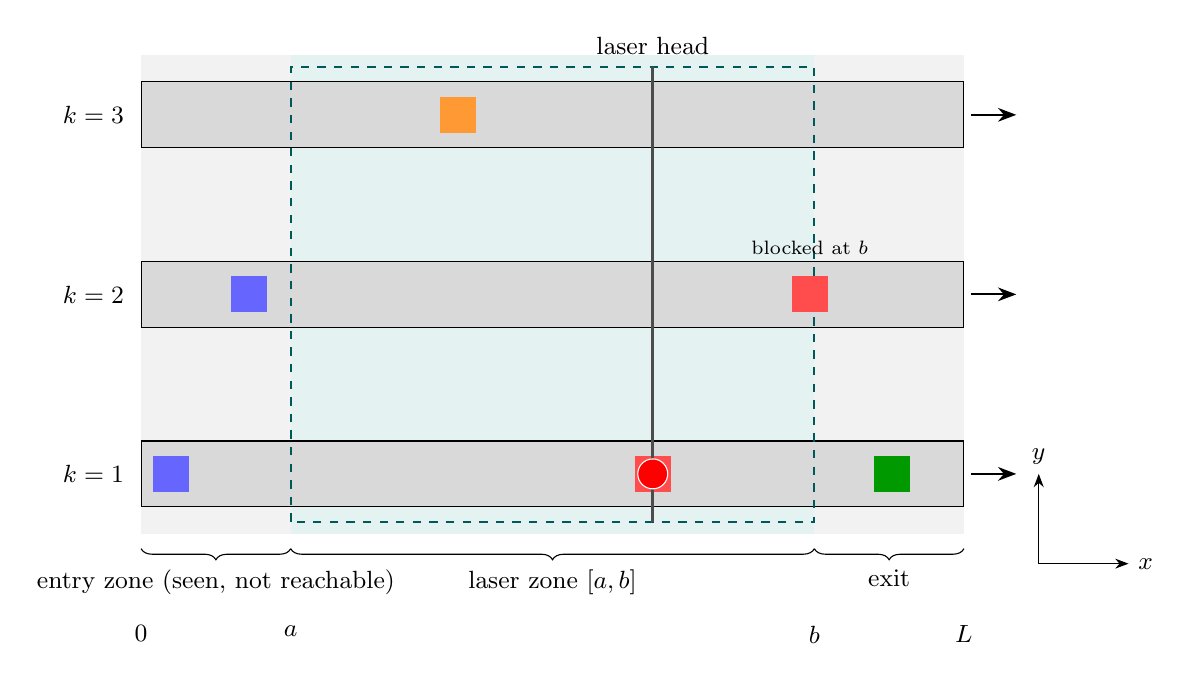
\begin{tikzpicture}[x=0.19cm,y=0.19cm,>=Stealth]
  \fill[gray!10] (0,-4) rectangle (10,28);
  \fill[teal!10] (10,-4) rectangle (45,28);
  \fill[gray!10] (45,-4) rectangle (55,28);
  \foreach \y/\n in {0/1,12/2,24/3}{
    \draw[fill=gray!30] (0,\y-2.2) rectangle (55,\y+2.2);
    \node[left] at (-0.5,\y) {\small $k=\n$};
    \draw[->,thick] (55.5,\y) -- (58.5,\y);
  }
  \draw[teal!70!black,dashed,thick] (10,-3.2) rectangle (45,27.2);
  \fill[blue!60] (0.8,-1.2) rectangle (3.2,1.2);
  \fill[blue!60] (6,10.8) rectangle (8.4,13.2);
  \fill[orange!80] (20,22.8) rectangle (22.4,25.2);
  \fill[red!70] (33,-1.2) rectangle (35.4,1.2);
  \fill[red!70] (43.5,10.8) rectangle (45.9,13.2);
  \fill[green!60!black] (49,-1.2) rectangle (51.4,1.2);
  \draw[very thick,gray!60!black] (34.2,-3.2) -- (34.2,27.2);
  \draw[fill=red,draw=white] (34.2,0) circle (1.0);
  \node[above] at (34.2,27.4) {\small laser head};
  \node[above,font=\scriptsize] at (44.7,14) {blocked at $b$};
  \draw[decorate,decoration={brace,mirror,amplitude=4pt}] (0,-5) -- (10,-5)
       node[midway,below=4pt] {\small entry zone (seen, not reachable)};
  \draw[decorate,decoration={brace,mirror,amplitude=4pt}] (10,-5) -- (45,-5)
       node[midway,below=4pt] {\small laser zone $[a,b]$};
  \draw[decorate,decoration={brace,mirror,amplitude=4pt}] (45,-5) -- (55,-5)
       node[midway,below=4pt] {\small exit};
  \node[below] at (0,-9.5) {\small $0$};
  \node[below] at (10,-9.5) {\small $a$};
  \node[below] at (45,-9.5) {\small $b$};
  \node[below] at (55,-9.5) {\small $L$};
  \draw[->] (60,-6) -- (66,-6) node[right] {\small $x$};
  \draw[->] (60,-6) -- (60,0) node[above] {\small $y$};
\end{tikzpicture}
\caption{The reference cell (top view). Parts travel in $+x$; the head reaches
$[a,b]\times[\min_k y_k,\max_k y_k]$ and is processing the part on belt~1 (red), whose
belt is stopped; the part on belt~2 has reached $b$ unprocessed and blocks its belt. The
controller sees the parts on the belts (entry and laser zones) but not the queue upstream
of the feed point.}
\label{fig:cell}
\end{figure}

\subsection{Objective and decision epochs}
An episode generates arrivals for a horizon $T_A$ (300~s) and runs until every part has
left. The objective is the \emph{penalized flow time}
\begin{equation}
J=\frac{1}{n}\sum_{j=1}^{n}(C_j-r_j)+\frac{\lambda_N N_B+\lambda_T T_B}{n},
\end{equation}
the mean flow time from arrival $r_j$ to completion $C_j$ plus a penalty for the $N_B$
blocking events and the $T_B$ conveyor-seconds stopped by blocking, with $\lambda_N=10$~s
per event and $\lambda_T=1$~s per conveyor-second (placeholders in equivalent seconds).
A decision epoch occurs whenever the head is free and at least one candidate exists; the
controller then chooses one candidate and the head commits to it. In the cell's basic
mode (\texttt{none}) the candidates are the parts inside the laser zone. In its design
mode (\texttt{when\_idle}) the head may also, when no part is in the zone, be sent to the
entry point $(a,y_k)$ of a belt on which a visible part approaches, and wait there; the
commitment is revoked at no cost if any part enters the zone, and the policy decides
again. Both modes are evaluated.

\subsection{Information}
The controller knows the time, the head's position and state, the state of every belt
(running, stopped for processing, blocked), and, for every part on a belt, its belt,
position, processing time and the instant from which it has been observed; it knows the
mean arrival rate of each belt and the arrival horizon, but never the future arrival
instants, and it does not see the parts queued upstream of the feed point. This is the
reference information model of the cell (an overhead camera over the belts); its
alternatives (no camera; a camera that also sees the upstream queue) are the subject of
Paper~2. Every policy below, including the look-ahead searches, uses only this
information: the simulator's look-ahead copy drops the real future arrivals and the
hidden queue, and a test verifies that changing them does not change any search cost.

\subsection{Properties}\label{sec:properties}
The formal model (belt odometers, exact continuous-time constraints, a time-indexed MILP
and a sequence-only decoder) is given in the project's formulation document; we state
here what matters for dispatching, with the proofs there.
\begin{itemize}[nosep]
\item \emph{Complexity.} With the number of conveyors $N$ part of the input and the
  processing stop limited to the part's own belt, the decision versions for $\sum_jC_j$
  (equivalently $\sum_jF_j$) and for $L_{\max}$ are strongly NP-hard, by reduction from
  $1\,|\,r_j\,|\,\sum C_j$ and $1\,|\,r_j\,|\,L_{\max}$ with one part per conveyor, where
  the head is the only coupling. A fixed $N$ with several parts per belt is not covered,
  nor is the makespan. In Graham notation the problem is a single machine with release
  dates, sequence-, time- and state-dependent setups (the travel to the interception
  point depends on the belt state, i.e.\ on every earlier stop), blocking and endogenous
  availability windows.
\item \emph{Belt order is not dominant.} On a conveyor the order of the parts never
  changes and the binding cap on the belt's advance is set by its most downstream
  unstarted part, so serving a conveyor out of belt order tends to cause blocking; yet on
  small instances with bursts the best order sometimes serves a later part first (gaps
  of 0.7--1.2\,\% on average and up to 3.5\,\% over all $n!$ orders of 6--7 parts), and on
  a single conveyor a short part behind a long one should go first (a counterexample
  with a 2~s per part difference). Policies restricted to belt heads form a restricted
  class; the policy of this paper points to any candidate.
\item \emph{Lower bounds.} Earliest-start bounds that account for the belt kinematics
  (the $m$-th part of a conveyor cannot be processed before the belt has advanced
  $a+(m-1)\delta$ after the first part's arrival, with the belt stopped during every
  forced processing), minimum gaps between two processings on the same or different
  conveyors, and a Jackson-type tail bound with travel are proved in the project's theory
  notes. They are used there to measure the quality of offline solutions on small
  instances; they do not enter the online method.
\item \emph{Light traffic.} When consecutive parts of a belt are far enough apart that
  no two are ever on the belt together and the head can always be in place, the schedule
  that processes every part at $x=a$ on arrival is optimal and the nearest-part, FIFO and
  nearest-head rules all attain it. The regimes of this paper are not in light traffic
  (processing loads 0.64 and 0.93), which is where the rules differ.
\end{itemize}

%====================================================================
\section{The look-ahead search}\label{sec:search}
%====================================================================

\subsection{Rollout over the known parts}
The first search is a fortified rollout \cite{M02_Bertsekas1997} on the cell's exact
event-driven simulator. At a decision epoch with candidate set $\mathcal C$ and base policy
$\mu$, it keeps the $K=6$ candidates with the smallest interception time, always
including $\mu$'s own choice; for each it clones the simulator with online information
only (the real future arrivals and the hidden queue removed), forces the candidate, lets
$\mu$ continue until every part known at the decision is processed, and scores the sum of
their completion times (the online counterpart of the mean flow time; blocking penalties
are not scored, which was better in every variant tried). It applies the best-scoring
first decision and re-plans at the next epoch, keeping the base choice on ties. With
$\mu=\nj$ it is the \emph{known-parts search} of the tables below; with $\mu$ equal to the
current network it is the teacher of the first training stage.

\subsection{Sampled futures, scored on every part}
The known-parts rollout has a ceiling: on the validation cells no network of any size
exceeded it by more than the noise (Section~\ref{sec:ladder}). The reason is its horizon.
The known parts are a few; the decision that serves them best may leave the head far from
the belt that will need it next, and the rollout cannot see that. The second search
samples the unknown future. For each candidate it runs $M$ look-aheads, each with a
different synthetic list of arrivals over the next $W$ seconds, Poisson at the belts'
known mean rates (the clone's horizon becomes $t+W$ and it drains after it), with common
random numbers: the same scenario index gives the same future to every candidate. The
score of a candidate is the mean over the $M$ futures of the \emph{realized cost of all
parts} from the decision on (the integral of work in progress, i.e.\ the sum of the flow
times of every part present or arriving), not the completion times of the known parts.
Table~\ref{tab:variants} gives the design study that led to $M=8$, $W=30$~s and no
penalty in the score, all variants run over the same trained S network on the same
development realizations (30 per group).

\begin{table}[t]
\centering\small
\caption{Teacher design study: paired $\Delta$ of the penalized flow time against \nj\
[\%, 95\,\% CI] of each look-ahead run over the trained S network of
Section~\ref{sec:ladder}, on the development realizations (real cell and heavy example,
30 each; 60 general cells), score = mean of the three; and seconds per episode. ``Penalty
in the cost'' scores the look-ahead on the penalized objective. Bold: the chosen teacher.}
\label{tab:variants}
\resizebox{\linewidth}{!}{% generated by experiments/paper1_figures.py
\begin{tabular}{@{}lccccc@{}}
\toprule
teacher over the trained S network & real & heavy & general & score & s / episode (real / heavy / general) \\
\midrule
network alone (no search) & $-4.55 \pm 1.88$ & $-2.52 \pm 2.26$ & $-1.59 \pm 1.42$ & -2.88 & 0.5 / 0.8 / 0.4 \\
known parts, $K=6$ & $-5.23 \pm 1.91$ & $-2.69 \pm 1.72$ & $-2.49 \pm 1.52$ & -3.47 & 2.0 / 7.2 / 3.0 \\
known parts, all candidates & $-5.23 \pm 1.91$ & $-2.69 \pm 1.72$ & $-2.49 \pm 1.52$ & -3.47 & 1.8 / 8.4 / 3.7 \\
value head at the first decision after $t+20$~s, 4 futures, penalty in the cost & $+18.14 \pm 4.48$ & $+37.94 \pm 2.95$ & $+22.82 \pm 7.48$ & +26.30 & 7.9 / 26.3 / 13.1 \\
value head at exactly $t+20$~s, 4 futures, penalty in the cost & $+54.36 \pm 7.75$ & $+67.01 \pm 5.36$ & $+37.66 \pm 10.71$ & +53.01 & 10.4 / 26.7 / 13.9 \\
1 sampled future, 30~s window, penalty in the cost & $-1.59 \pm 2.04$ & $+6.73 \pm 2.12$ & $+2.82 \pm 2.79$ & +2.65 & 5.7 / 18.5 / 8.1 \\
2 sampled futures, 30~s window, penalty in the cost & $-4.11 \pm 1.73$ & $+0.47 \pm 1.42$ & $+0.12 \pm 2.03$ & -1.17 & 7.8 / 25.9 / 12.2 \\
4 sampled futures, 30~s window, penalty in the cost & $-6.68 \pm 1.93$ & $-1.40 \pm 1.76$ & $-0.94 \pm 1.79$ & -3.01 & 11.9 / 45.5 / 23.4 \\
4 sampled futures, 30~s window & $-6.67 \pm 1.78$ & $-3.52 \pm 1.51$ & $-3.00 \pm 1.53$ & -4.40 & 11.8 / 46.1 / 23.3 \\
4 sampled futures, 20~s window & $-6.60 \pm 1.85$ & $-3.82 \pm 1.47$ & $-2.43 \pm 1.68$ & -4.28 & 10.5 / 36.8 / 19.6 \\
4 sampled futures, 45~s window & $-6.85 \pm 2.14$ & $-3.65 \pm 1.35$ & $-2.20 \pm 1.37$ & -4.23 & 18.3 / 68.0 / 33.2 \\
4 sampled futures, 60~s window, penalty in the cost & $-4.66 \pm 1.93$ & $-0.23 \pm 1.64$ & $-0.49 \pm 1.79$ & -1.79 & 20.2 / 77.9 / 39.0 \\
6 sampled futures, 30~s window & $-6.51 \pm 1.94$ & $-4.01 \pm 1.46$ & $-2.96 \pm 1.52$ & -4.49 & 19.0 / 78.1 / 39.7 \\
8 sampled futures, 30~s window & $-7.50 \pm 1.92$ & $-3.83 \pm 1.33$ & $-3.19 \pm 1.53$ & \textbf{-4.84} & 21.9 / 112.2 / 58.3 \\
8 sampled futures, 20~s window & $-7.39 \pm 1.83$ & $-3.53 \pm 1.57$ & $-3.15 \pm 1.51$ & -4.69 & 17.7 / 85.9 / 42.4 \\
4 sampled futures, 30~s window, all candidates & $-6.67 \pm 1.78$ & $-3.52 \pm 1.51$ & $-3.00 \pm 1.53$ & -4.40 & 13.3 / 87.6 / 30.9 \\
4 sampled futures, 30~s window, half-weight penalty & $-7.24 \pm 1.54$ & $-3.43 \pm 1.38$ & $-2.97 \pm 1.62$ & -4.54 & 14.6 / 50.3 / 14.9 \\
\bottomrule
\end{tabular}
}
\end{table}

Four findings fix the design. (i) \emph{Sampled futures help only when the objective
counts every part.} An earlier attempt added four futures to the known-parts score and
was much worse than no futures at all ($+7.9$ against $-3.8$\,\% on the real cell): with
synthetic arrivals in the clone and only the known parts in the score, the look-ahead
rewards starving the new parts. With the all-parts score, four futures already beat the
known-parts rollout in every group, and eight gain another half point. (ii) \emph{One or
two futures are worse than none}: the sampled future is noise until it is averaged.
(iii) \emph{Window.} 20--30~s is best; 45--60~s add noise faster than information, since
the futures diverge from each other. (iv) \emph{Truncating the look-ahead with a learned
value is far worse than not truncating.} Cutting each rollout at $t+20$~s and adding the
value head's estimate of the cost-to-go gives $+18$ to $+54$\,\% against \nj: the
cost-to-go depends mostly on the random future arrivals, so its scale (hundreds of
part-seconds) and the value head's error (a quarter of that scale) are far larger than
the differences between candidates (seconds). Cutting at a fixed instant, where the
errors should be correlated across candidates, is even worse than cutting at a decision,
because the value head was trained on decision states only. We therefore run every
look-ahead to the end of its window and drain. The penalty in the score hurts here as it
did in every earlier version of the cell's rollout; a flow-time look-ahead ranks the
candidates better even though the policies are judged on the penalized objective.

The cost of the chosen teacher is about ten times that of the known-parts rollout per
episode: 22~s on the real cell and 112~s on the heavy example on one worker, i.e.\
0.4--1.9~s per decision (Section~\ref{sec:confirm}). It is a teacher, not a controller.

%====================================================================
\section{The learned policy}\label{sec:policy}
%====================================================================

\subsection{State as a set of tokens}
The policy reads the decision state as an unordered set of tokens: one per unfinished
part on a belt or being processed (23 features: status, position and distance to $b$,
time to $b$ at belt speed, interception time from the head and a reachability flag,
waiting time since the part became observable, processing time and remaining processing,
blocking flag, rank on the belt and a head flag, candidate and committed flags, offsets
from the head, its belt's speed and state), one per conveyor (11 features: offset from the
head, speeds, running, stopped, blocked, queue lengths on the belt, arrival rate, offered
load, has a candidate), one for the head (9: position, state, remaining processing,
commitment) and one context token (21: head speeds and motion model, mean processing
time, total offered load, geometry, pre-positioning mode, penalty weights, whether
arrivals are still coming and the time left to the horizon, numbers of parts and
candidates). Lengths are scaled by the belt length, speeds by 3~cm/s, times through
$\mathrm{sign}(t)\log(1+|t|/10\,\mathrm{s})$, which keeps long waits at heavy load bounded
and distinguishable. No token holds a list position or a conveyor index: a part is linked
to its belt through its $y$ offset and a copy of its belt's state. Encoding takes
0.14--0.19~ms per decision.

\subsection{Network}
One linear embedding per token type to width $d$, plus a learned type vector; a pre-norm
Transformer encoder with ReLU feed-forward blocks and no positional encoding, so that the
output is permutation-equivariant in the parts and the conveyors; a global vector $g$ as
the masked mean over all tokens. The policy head gives a logit $\mathrm{MLP}([h_i,g])$ to
every part token; non-candidates and padding receive $-\infty$, so the action is a
pointer to \emph{any} candidate of the open decision, not only a belt head. A value head
$\mathrm{MLP}([g,h_{\mathrm{ctx}},h_{\mathrm{head}}])$ predicts the normalized cost-to-go
(used in training only). Size S has 4 layers, $d=128$, 4 heads, 0.88~M parameters; M
has 8 layers, $d=256$, 8 heads, 6.7~M; L has 12 layers, $d=512$, 8 heads, 39~M. Tests
check permutation invariance (shuffled tokens give identically permuted logits and the
same value), exact masking, batch consistency, and that an untrained network drives valid
episodes. Single-state inference on one thread takes 4.1~ms (median) for S, 15~ms for M
and 64~ms for L on an unloaded machine; S is the size that fits a 5~ms budget, and
Section~\ref{sec:ladder} shows that the others do not decide better.

\subsection{Expert iteration}
Training alternates data generation and fitting. In iteration 0 the known-parts rollout
over \nj\ acts (with 10\,\% random actions for coverage) on episodes drawn from the
training distribution of Section~\ref{sec:dist} and labels every decision with at least
two candidates with the look-ahead costs of its candidates; the network is trained from
scratch on them. In iteration $k\ge1$ the teacher is the search over $\mathrm{net}_{k-1}$,
the acting policy is $\mathrm{net}_{k-1}$ except that the teacher acts with probability
$\beta=0.3$, and $\mathrm{net}_k$ is fine-tuned from $\mathrm{net}_{k-1}$ on a replay
buffer of the last two iterations. The policy loss is the cross-entropy to the softmin of
the relative look-ahead costs with temperature 1~s (a candidate 1~s worse than the best
gets $e^{-1}$ of its weight), the value loss $0.25\times$ the MSE of the normalized
cost-to-go; AdamW, one-cycle learning rate ($10^{-3}$ from scratch, $3\cdot10^{-4}$ when
fine-tuning), batch 256, gradient clipping at 1. After each iteration the network and
its teacher are scored on fixed validation cells (the real cell, its heavy variant, a set
of general cells and, from the last run on, the real cell with bursts; 50 realizations
per group, 100 general cells), by the mean paired $\Delta$ of the penalized flow time
against \nj; the network is kept only if the mean over the groups improves, and the run
stops after two rejections. Seeds, arguments, machine, times, losses and validation of
every run are logged and distributed with the models.

\subsection{Training distribution}\label{sec:dist}
Every training episode draws one cell: the real cell (25\,\%), its heavy variant
(10\,\%), or a general cell (65\,\%) with $N\in\{1,\dots,6\}$ conveyors, belt speeds
$U[1.5,6]$~cm/s per belt, a processing load $\rho_p\sim U[0.3,0.95]$ split between the
belts, mean processing time $U[1.5,4]$~s with constant, uniform or normal distributions,
head speeds $U[5,20]$~cm/s per axis (with probability 0.3, $U[2.5,5]$), simultaneous or
sequential axes, every geometric length scaled by $U[0.5,1.5]$ of the real value, penalty
weights $\lambda_N\sim U[0,20]$~s and $\lambda_T\sim U[0,2]$, the stop rule (own belt or
all belts), the pre-positioning mode (half and half), the observation level (the
reference model 70\,\%, no camera 15\,\%, the hidden queue visible 15\,\%) and, with
probability 0.5, bursty arrivals. All values reach the network through its tokens except
the burst parameters, which it must infer from what it sees. Training seeds (100\,000+)
and validation seeds (2\,000+, 2\,500+) are disjoint from each other and from the reserved
seeds of Section~\ref{sec:confirm}.

%====================================================================
\section{Development results}\label{sec:dev}
%====================================================================
Everything in this section was measured on development realizations and used to make
design decisions; nothing here is confirmatory.

\subsection{Three sizes, one teacher: the ladder stops at S}\label{sec:ladder}
With the known-parts teacher, the three sizes were trained on a 48-thread workstation
with one GPU, same code, same seeds, same gating, with the data scaled with the size
(Table~\ref{tab:ladder}, Figure~\ref{fig:training} left). Every network alone beats its
rule teacher at the real load and generalizes to the general cells, where \nh\ loses; the
search over each network saturates from iteration 1 at $-4.7$ to $-5.1$\,\% on the real
cell, and from iteration 2 each network is within 0.3--0.7 points of its own teacher. The
best scores are $-2.79$\,\% (S, iteration 3), $-2.88$\,\% (M, iteration 3) and $-2.44$\,\%
(L, iteration 1, after 14~h), all within the confidence intervals of one another. Training
losses keep falling while validation stalls: the networks fit their teacher ever better,
and the teacher is the ceiling. M costs $8.5\times$ more per generated episode and
$4\times$ more per decision than S for no measurable gain; L is not under-fitted by lack
of data (it had four times S's) but learns the same teacher more slowly. The ladder stops
at S, and the lever is the teacher.

\begin{table}[t]
\centering\small
\caption{Scaling ladder with the known-parts teacher: best accepted iteration of each
run on the validation groups (paired $\Delta$ vs \nj\ [\%, 95\,\% CI]; 50 realizations
for the real cell and the heavy example, 100 general cells) and the score of the search
over that network.}
\label{tab:ladder}
\resizebox{\linewidth}{!}{% generated by experiments/paper1_figures.py
\begin{tabular}{@{}llcccccccc@{}}
\toprule
run & size & params & episodes it.\ 0 / later & best it. & net real & net heavy & net general & score & search over net (score) \\
\midrule
\texttt{rl2\_gen\_s\_big} & S & 0.88 M & 4000 / 2000 & 3 of 5 & $-4.42 \pm 1.44$ & $-2.32 \pm 1.63$ & $-1.64 \pm 1.06$ & -2.79 & -3.10 \\
\texttt{rl2\_gen\_m} & M & 6.7 M & 8000 / 4000 & 3 of 5 & $-4.49 \pm 1.55$ & $-2.22 \pm 1.38$ & $-1.91 \pm 1.08$ & -2.88 & -3.18 \\
\texttt{rl2\_gen\_l} & L & 39 M & 16000 / 8000 & 1 of 1 & $-4.25 \pm 1.53$ & $-1.67 \pm 1.32$ & $-1.40 \pm 1.04$ & -2.44 & -2.96 \\
\bottomrule
\end{tabular}
}
\end{table}

\begin{figure}[t]
\centering
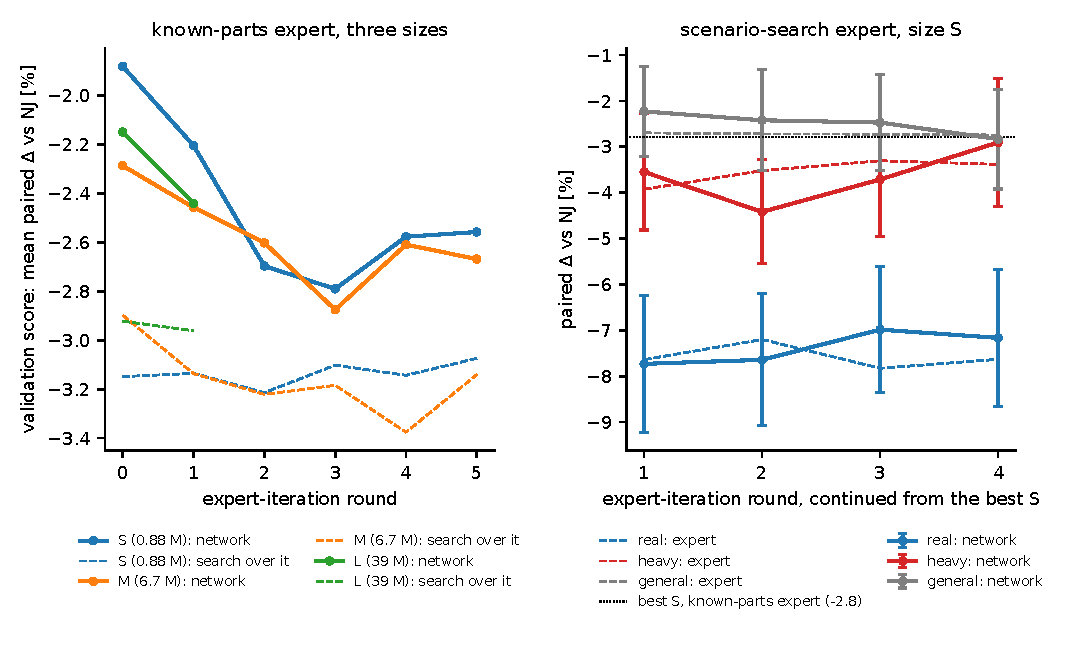
\includegraphics[width=\linewidth]{figures/training.pdf}
\caption{Left: validation score (mean paired $\Delta$ vs \nj\ over the three groups) per
expert-iteration round for the three sizes with the known-parts teacher (solid: network
alone; dashed: the search over it). Right: the S network continued with the sampled-future
teacher, per group (network alone with 95\,\% CIs; dashed: its teacher); the dotted line is
the best S score with the known-parts teacher.}
\label{fig:training}
\end{figure}

\subsection{The sampled-future teacher raises the ceiling}\label{sec:sf}
Continuing the best S network with the sampled-future teacher (Table~\ref{tab:sfruns},
Figure~\ref{fig:training} right) moved the score from $-2.79$ to $-4.50$\,\% after one
iteration and $-4.83$\,\% after two: $-7.6$\,\% on the real cell, $-4.4$\,\% on the heavy
example and $-2.4$\,\% on the general cells, at the same 4~ms per decision. From the second
iteration the network alone is at or above the search over itself on the real and heavy
cells ($-7.6$ against $-7.2$, $-4.4$ against $-3.5$): the search is noisy (eight sampled
futures) and the network learns its average. Two further continuations changed the
training set rather than the method: the design mode with its corrected tokens and the
three observation levels (score $-3.98$\,\% in the design mode, where the \nj\ baseline
already pre-positions), and bursty arrivals with slow heads in the mix (score
$-3.82$\,\% over four groups). The last network is indistinguishable from the previous
one head to head ($+0.47\pm0.69$, $-0.36\pm0.83$, $+0.20\pm0.48$ and $+0.09\pm0.36$\,\% on
the four groups): extending the training to the declared scope produced no detectable
improvement, and the owner froze that network (iteration~1) for the confirmatory run.

\begin{table}[t]
\centering\small
\caption{Expert iteration with the sampled-future teacher, size S: per iteration, the
network alone on the validation groups (paired $\Delta$ vs \nj\ [\%, 95\,\% CI]), its
score and its teacher's score. Bold iterations were accepted. The first run validates in
the basic mode; the two continuations in the design mode (where \nj\ also
pre-positions), with the fourth group added in the last.}
\label{tab:sfruns}
\resizebox{\linewidth}{!}{% generated by experiments/paper1_figures.py
\begin{tabular}{@{}llcccccc@{}}
\toprule
run & it. & net real & net heavy & net general & net real/bursts & score & teacher score \\
\midrule
\multicolumn{8}{@{}l}{\texttt{rl2\_gen\_s\_sf}: sampled-future teacher, from \texttt{rl2\_gen\_s\_big}; `none'} \\
 & \textbf{1} & $-7.73 \pm 1.49$ & $-3.55 \pm 1.26$ & $-2.23 \pm 0.98$ & --- & -4.50 & -4.75 \\
 & \textbf{2} & $-7.64 \pm 1.44$ & $-4.42 \pm 1.13$ & $-2.42 \pm 1.10$ & --- & -4.83 & -4.48 \\
 & 3 & $-6.99 \pm 1.38$ & $-3.71 \pm 1.25$ & $-2.47 \pm 1.05$ & --- & -4.39 & -4.62 \\
 & 4 & $-7.16 \pm 1.48$ & $-2.91 \pm 1.40$ & $-2.83 \pm 1.09$ & --- & -4.30 & -4.59 \\
\multicolumn{8}{@{}l}{\texttt{rl2\_gen\_s\_d}: + design mode, corrected tokens, observation levels; from \texttt{s\_sf}} \\
 & \textbf{1} & $-6.40 \pm 1.50$ & $-2.04 \pm 1.28$ & $-3.08 \pm 1.08$ & --- & -3.84 & -4.15 \\
 & \textbf{2} & $-6.61 \pm 1.40$ & $-2.45 \pm 1.20$ & $-2.88 \pm 1.07$ & --- & -3.98 & -4.35 \\
 & 3 & $-6.67 \pm 1.36$ & $-2.40 \pm 1.32$ & $-2.87 \pm 1.06$ & --- & -3.98 & -4.00 \\
 & 4 & $-6.37 \pm 1.43$ & $-2.45 \pm 1.32$ & $-2.82 \pm 1.05$ & --- & -3.88 & -4.20 \\
\multicolumn{8}{@{}l}{\texttt{rl2\_gen\_s\_b}: + bursts and slow heads in the mix; from \texttt{s\_d}} \\
 & \textbf{1} & $-6.19 \pm 1.48$ & $-2.86 \pm 1.09$ & $-2.73 \pm 1.05$ & $-3.51 \pm 1.00$ & -3.82 & -4.09 \\
 & 2 & $-6.20 \pm 1.36$ & $-2.60 \pm 1.23$ & $-2.73 \pm 1.06$ & $-3.66 \pm 0.99$ & -3.80 & -3.98 \\
 & 3 & $-6.48 \pm 1.45$ & $-2.25 \pm 1.06$ & $-2.72 \pm 1.08$ & $-3.74 \pm 0.92$ & -3.80 & -3.99 \\
\bottomrule
\end{tabular}
}
\end{table}

\subsection{A burst-aware teacher does not help}\label{sec:futures}
A network trained on bursty cells cannot exceed a teacher whose futures are Poisson, so
the natural next lever was a teacher that samples the cell's on/off arrival model
(statistical knowledge of the process, started in its stationary state, not an
observation of the source's current state). Table~\ref{tab:futures} tests it on the
frozen network, the same realizations and the same budget. On Poisson cells the two
teachers coincide by construction; on the bursty cell the burst-aware teacher is half a
point \emph{worse} ($+0.52\pm0.49$\,\% paired against the Poisson one), and with strong
bursts the two are equal within $\pm0.4$--$0.6$ points. The stationary start adds to
every future the uncertainty of whether the source is emitting now, which eight futures
do not average out; the smoother Poisson future ranks the candidates with less noise. With
strong bursts the cell alternates between an idle head and a saturated burst, no teacher
beats the network, and the known-parts order is close to what can be achieved without
seeing the hidden queue. The Poisson teacher stays the teacher of record.

\begin{table}[t]
\centering\small
\caption{Teacher futures: the frozen network alone, and the sampled-future search over
it with Poisson futures and with the cell's on/off arrival model, on the validation
groups (design mode, 50 realizations per group, 100 general) and on two cells with
strong bursts (on 20\,\% of the time in 40~s periods). Paired $\Delta$ vs \nj\ [\%,
95\,\% CI].}
\label{tab:futures}
\resizebox{\linewidth}{!}{% generated by experiments/paper1_figures.py
\begin{tabular}{@{}lcccccc@{}}
\toprule
policy & real & heavy & general & real, bursts (0.3 / 20 s) & heavy, strong bursts (0.2 / 40 s) & real, strong bursts \\
\midrule
network alone & $-6.19 \pm 1.48$ & $-2.86 \pm 1.09$ & $-2.73 \pm 1.05$ & $-3.51 \pm 1.00$ & $-1.06 \pm 0.61$ & $-1.85 \pm 0.75$ \\
teacher, Poisson futures & $-6.44 \pm 1.30$ & $-2.35 \pm 1.46$ & $-3.51 \pm 1.27$ & $-4.07 \pm 0.96$ & $-1.13 \pm 0.58$ & $-1.60 \pm 0.71$ \\
teacher, cell futures & $-6.44 \pm 1.30$ & $-2.35 \pm 1.46$ & $-3.51 \pm 1.27$ & $-3.60 \pm 0.89$ & $-1.27 \pm 0.61$ & $-1.56 \pm 0.69$ \\
\bottomrule
\end{tabular}
}
\end{table}

%====================================================================
\section{Confirmatory evaluation}\label{sec:confirm}
%====================================================================

\subsection{Protocol}
The frozen network, the known-parts search over \nj, the sampled-future search over the
network (the teacher), \nj\ and \nh\ were run on 30 realizations reserved for this
evaluation (seeds 7000--7029), never seen by any design decision and used once, on eight
regimes: the real cell and its heavy variant, Poisson and bursty arrivals, nominal head
and a head twice as slow (Table~\ref{tab:regimes}), in the basic mode (B) and in the
design mode (C). Every policy runs on the same realizations (common random numbers), so
every contrast is a paired difference; we report $\Delta=100\,(\frac{1}{30}\sum_\omega
J_X(\omega)/J_Y(\omega)-1)$ for ``X vs Y'', negative favouring $X$, with a normal 95\,\%
interval and, for the contrasts between policies, the number of realizations in which $X$
is cheaper. Latencies are measured on the decisions of the network's episodes: at every
decision with at least two candidates, every policy is timed on the same state (one
thread, the machine fully loaded by the other workers), 16\,215 decisions in B and
17\,147 in C. The protocol, the regimes and the contrasts were fixed before the run; the
per-episode results and the per-decision latencies are distributed with the source.

\begin{table}[t]
\centering\small
\caption{Regimes of the confirmatory evaluation and their physical scales ($\tcross$ is
the head's travel time across the conveyors); parts, penalized flow time, flow time,
blocking events and blocked conveyor-seconds are means per episode for \nj\ in B over the
30 realizations.}
\label{tab:regimes}
\resizebox{\linewidth}{!}{% generated by experiments/paper1_figures.py
\begin{tabular}{@{}lcccccccc@{}}
\toprule
regime & belt [cm/s] & head [cm/s] & $\tau_{\mathrm{cross}}$ [s] & parts & $J$ (\textsc{nj}, B) [s/part] & flow [s] & blocking events & blocked [belt-s] \\
\midrule
real / Poisson / nominal head & 3 & 10 & 2.4 & 78 & 21.8 & 19.3 & 7.8 & 122 \\
real / Poisson / slow head & 3 & 5 & 4.8 & 78 & 42.1 & 36.1 & 14.8 & 322 \\
real / bursts / nominal head & 3 & 10 & 2.4 & 73 & 27.6 & 25.8 & 5.1 & 93 \\
real / bursts / slow head & 3 & 5 & 4.8 & 73 & 41.3 & 37.8 & 8.2 & 184 \\
heavy / Poisson / nominal head & 5 & 5 & 4.8 & 94 & 73.5 & 65.2 & 18.2 & 601 \\
heavy / Poisson / slow head & 5 & 2.5 & 9.6 & 94 & 104.0 & 94.7 & 14.2 & 720 \\
heavy / bursts / nominal head & 5 & 5 & 4.8 & 89 & 72.0 & 66.4 & 11.1 & 399 \\
heavy / bursts / slow head & 5 & 2.5 & 9.6 & 89 & 93.6 & 87.0 & 9.1 & 508 \\
\bottomrule
\end{tabular}
}
\end{table}

\subsection{Results}
Table~\ref{tab:confirmB} and Figure~\ref{fig:confirm} give the basic mode;
Table~\ref{tab:confirmC} the design mode; Table~\ref{tab:latency} the latencies.

\begin{table}[t]
\centering\small
\caption{Confirmatory evaluation, basic mode (B): paired $\Delta$ of the penalized flow
time of each policy against \nj; contrasts of the two searches against the network
(positive = the network is better; in parentheses the realizations in which the search
is cheaper); and per-decision latency (median / 95th percentile). Bold: the interval
excludes zero.}
\label{tab:confirmB}
\resizebox{\linewidth}{!}{% generated by experiments/paper1_figures.py
\begin{tabular}{@{}lccc|cc|ccc@{}}
\toprule
 & \multicolumn{3}{c|}{paired $\Delta$ vs \textsc{nj} [\%]} & \multicolumn{2}{c|}{contrasts [\%]} & \multicolumn{3}{c}{latency p50 / p95 [ms]} \\
regime & known-parts & sampled-future & network & search vs net & teacher vs net & search & network & teacher \\
\midrule
real / Poisson / nominal head & {\boldmath$-4.16 \pm 1.98$} & {\boldmath$-7.60 \pm 2.17$} & {\boldmath$-7.22 \pm 1.95$} & {\boldmath$+3.35 \pm 1.10$} (1/30) & $-0.39 \pm 1.24$ (17/30) & 2.0 / 6.9 & 8.5 / 13.7 & 0.43 / 1.43 s \\
real / Poisson / slow head & {\boldmath$-3.73 \pm 2.17$} & {\boldmath$-7.72 \pm 2.14$} & {\boldmath$-7.25 \pm 1.74$} & {\boldmath$+3.83 \pm 1.56$} (3/30) & $-0.53 \pm 1.12$ (15/30) & 3.3 / 10.5 & 10.2 / 15.3 & 0.82 / 2.22 s \\
real / bursts / nominal head & $-0.57 \pm 1.54$ & {\boldmath$-2.68 \pm 1.44$} & {\boldmath$-1.96 \pm 1.74$} & $+1.54 \pm 1.60$ (6/30) & $-0.65 \pm 1.12$ (16/30) & 4.3 / 12.6 & 9.8 / 14.7 & 0.84 / 2.31 s \\
real / bursts / slow head & {\boldmath$-4.25 \pm 1.91$} & {\boldmath$-6.72 \pm 2.12$} & {\boldmath$-6.24 \pm 2.00$} & {\boldmath$+2.22 \pm 1.42$} (7/30) & $-0.48 \pm 1.22$ (16/30) & 5.1 / 13.4 & 10.9 / 16.2 & 1.14 / 2.67 s \\
heavy / Poisson / nominal head & $+0.26 \pm 1.45$ & {\boldmath$-3.68 \pm 1.58$} & {\boldmath$-2.78 \pm 1.85$} & {\boldmath$+3.31 \pm 1.87$} (9/30) & $-0.81 \pm 1.46$ (16/30) & 5.0 / 14.9 & 11.3 / 17.5 & 1.37 / 3.33 s \\
heavy / Poisson / slow head & $+2.31 \pm 2.94$ & $-1.40 \pm 2.53$ & $-1.32 \pm 2.32$ & {\boldmath$+3.86 \pm 2.86$} (9/30) & $+0.05 \pm 2.24$ (15/30) & 5.6 / 15.9 & 11.7 / 18.0 & 1.47 / 3.54 s \\
heavy / bursts / nominal head & $-1.02 \pm 1.33$ & {\boldmath$-3.56 \pm 1.74$} & {\boldmath$-3.29 \pm 1.66$} & {\boldmath$+2.46 \pm 1.36$} (2/30) & $-0.27 \pm 0.55$ (17/30) & 7.3 / 21.3 & 12.2 / 19.6 & 1.86 / 5.12 s \\
heavy / bursts / slow head & {\boldmath$-1.89 \pm 1.87$} & {\boldmath$-4.15 \pm 1.82$} & {\boldmath$-4.15 \pm 1.74$} & {\boldmath$+2.40 \pm 1.29$} (6/30) & $+0.01 \pm 0.79$ (18/30) & 6.3 / 19.9 & 11.4 / 18.6 & 1.58 / 4.44 s \\
\bottomrule
\end{tabular}
}
\end{table}

\begin{table}[t]
\centering\small
\caption{As Table~\ref{tab:confirmB}, design mode (C): every policy, including \nj, may
pre-position the idle head.}
\label{tab:confirmC}
\resizebox{\linewidth}{!}{% generated by experiments/paper1_figures.py
\begin{tabular}{@{}lccc|cc|ccc@{}}
\toprule
 & \multicolumn{3}{c|}{paired $\Delta$ vs \textsc{nj} [\%]} & \multicolumn{2}{c|}{contrasts [\%]} & \multicolumn{3}{c}{latency p50 / p95 [ms; teacher in s]} \\
regime & known-parts & sampled-future & network & search vs net & teacher vs net & search & network & teacher \\
\midrule
real / Poisson / nominal head & {\boldmath$-3.61 \pm 2.18$} & {\boldmath$-6.83 \pm 2.40$} & {\boldmath$-7.08 \pm 2.18$} & {\boldmath$+3.85 \pm 1.61$} (4/30) & $+0.27 \pm 1.04$ (13/30) & 1.8 / 7.5 & 8.5 / 13.4 & 0.39 / 1.50 s \\
real / Poisson / slow head & {\boldmath$-3.06 \pm 2.68$} & {\boldmath$-7.09 \pm 2.60$} & {\boldmath$-7.02 \pm 2.70$} & {\boldmath$+4.44 \pm 2.07$} (5/30) & $+0.04 \pm 1.69$ (16/30) & 3.3 / 9.8 & 9.9 / 15.2 & 0.77 / 2.03 s \\
real / bursts / nominal head & $-0.74 \pm 1.10$ & {\boldmath$-2.33 \pm 1.10$} & {\boldmath$-2.04 \pm 1.05$} & {\boldmath$+1.37 \pm 1.09$} (7/30) & $-0.28 \pm 0.78$ (12/30) & 2.9 / 12.0 & 9.9 / 15.0 & 0.57 / 2.29 s \\
real / bursts / slow head & {\boldmath$-3.11 \pm 2.13$} & {\boldmath$-7.32 \pm 2.18$} & {\boldmath$-6.56 \pm 2.15$} & {\boldmath$+3.85 \pm 2.01$} (8/30) & $-0.77 \pm 0.99$ (18/30) & 4.3 / 13.3 & 10.5 / 16.2 & 0.97 / 2.72 s \\
heavy / Poisson / nominal head & $-0.86 \pm 1.82$ & {\boldmath$-3.91 \pm 1.73$} & {\boldmath$-4.14 \pm 1.62$} & {\boldmath$+3.49 \pm 1.53$} (7/30) & $+0.27 \pm 1.08$ (12/30) & 4.8 / 13.6 & 11.1 / 17.3 & 1.30 / 3.20 s \\
heavy / Poisson / slow head & $+0.42 \pm 1.94$ & $-0.10 \pm 2.05$ & $-1.64 \pm 2.72$ & $+2.52 \pm 2.73$ (10/30) & $+1.98 \pm 2.75$ (12/30) & 5.8 / 17.8 & 11.6 / 17.9 & 1.52 / 4.00 s \\
heavy / bursts / nominal head & {\boldmath$-2.21 \pm 1.37$} & {\boldmath$-4.78 \pm 1.50$} & {\boldmath$-4.53 \pm 1.38$} & {\boldmath$+2.47 \pm 0.95$} (3/30) & $-0.25 \pm 0.79$ (15/30) & 6.4 / 19.8 & 11.9 / 18.7 & 1.66 / 4.59 s \\
heavy / bursts / slow head & {\boldmath$-3.06 \pm 1.95$} & {\boldmath$-4.96 \pm 1.78$} & {\boldmath$-4.56 \pm 2.00$} & {\boldmath$+1.67 \pm 1.47$} (7/30) & $-0.32 \pm 1.25$ (16/30) & 6.0 / 19.4 & 11.0 / 18.2 & 1.44 / 4.12 s \\
\bottomrule
\end{tabular}
}
\end{table}

\begin{figure}[t]
\centering
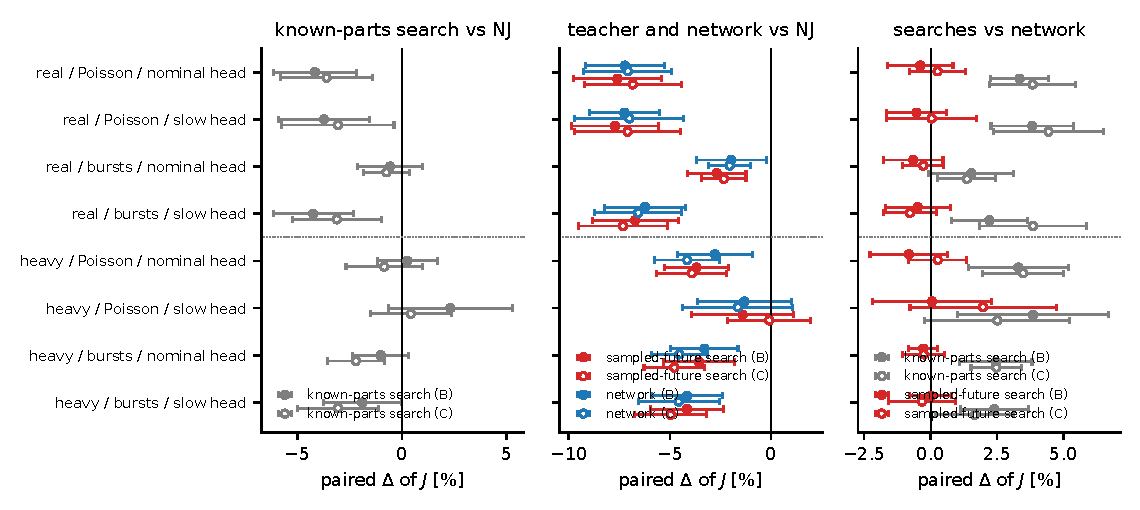
\includegraphics[width=\linewidth]{figures/confirm.pdf}
\caption{Confirmatory evaluation on the eight regimes (paired $\Delta$ of the penalized
flow time, 95\,\% CI; filled markers: basic mode B, hollow: design mode C). Left: the
known-parts search against \nj. Middle: the sampled-future search (teacher) and the
network against \nj. Right: the two searches against the network (positive = the network
is better).}
\label{fig:confirm}
\end{figure}

\begin{table}[t]
\centering\small
\caption{Per-decision latency of every policy on the same decisions (one thread, machine
fully loaded), pooled over the eight regimes: 16\,215 decisions in B, 17\,147 in C.}
\label{tab:latency}
\resizebox{\linewidth}{!}{% generated by experiments/paper1_figures.py
\begin{tabular}{@{}lcccc|cccc@{}}
\toprule
 & \multicolumn{4}{c|}{treatment B [ms]} & \multicolumn{4}{c}{treatment C [ms]} \\
policy & p50 & p95 & p99 & max & p50 & p95 & p99 & max \\
\midrule
\textsc{nj} & 0.07 & 0.17 & 0.28 & 3.3 & 0.06 & 0.16 & 0.28 & 9.9 \\
\textsc{nh} & 0.01 & 0.07 & 0.14 & 4.7 & 0.01 & 0.06 & 0.13 & 1.2 \\
known-parts search & 4.78 & 15.99 & 24.42 & 54.1 & 4.40 & 15.56 & 23.08 & 83.6 \\
network & 10.83 & 17.53 & 25.46 & 105.9 & 10.65 & 17.19 & 24.43 & 88.2 \\
sampled-future search & 1178.59 & 3630.54 & 5385.06 & 12159.0 & 1073.71 & 3511.40 & 5094.76 & 12039.6 \\
\bottomrule
\end{tabular}
}
\end{table}

\textbf{The network alone beats \nj\ in seven of the eight regimes}, by 2.0--7.3\,\% in B
($-7.2$ and $-7.3$\,\% on the real cell with Poisson arrivals, $-2.0$ and $-6.2$ with
bursts, $-2.8$ to $-4.2$ at the heavy load) and by 2.0--7.1\,\% in C; the exception is the
heavy load with Poisson arrivals and a slow head ($-1.3\pm2.3$ and $-1.6\pm2.7$), where
with every belt queueing and a head at 2.5~cm/s the nearest-part rule is close to the
best one can do without seeing the queues.

\textbf{It beats the known-parts search in every regime}, by 1.5--3.9 points in B and
1.4--4.4 in C, significantly in seven of eight in both modes, at 2--3 times the search's
latency. The known-parts search is not a competitive reference at the heavy load
($+0.3$ and $+2.3$\,\% against \nj\ with Poisson arrivals in B): the look-ahead over the
parts in view, without the sampled future, ranks the candidates worse than the rule when
every belt is queueing.

\textbf{It equals its teacher.} The sampled-future search over the network is within
$\pm0.8$ points of the network alone in every regime and mode, never significantly
better (it is cheaper in 12--18 of the 30 realizations), at 0.4--1.9~s per decision
(median by regime; 1.2~s pooled, 3.6~s at the 95th percentile, 12~s at most; 2\,600
look-aheads per episode on average). The amortized policy recovers the search at about
1/100 of its latency, on reserved realizations, which is what every development run had
shown on the validation cells.

\textbf{Latency.} Pooled over the regimes, the network decides in 10.8~ms (median),
17.5~ms (95th percentile), 25.5~ms (99th) and 106~ms at most, on one thread with the
machine fully loaded by 47 other workers (Figure~\ref{fig:latency}); the 4~ms of
Section~\ref{sec:policy} is the same model on an unloaded machine. The physical slack of
the cell, the time until the next part reaches $b$, is seconds, three orders of magnitude
above either figure. The known-parts search decides in 4.8~ms (16~ms at the 95th
percentile) and the rules in under 0.2~ms.

\begin{figure}[t]
\centering
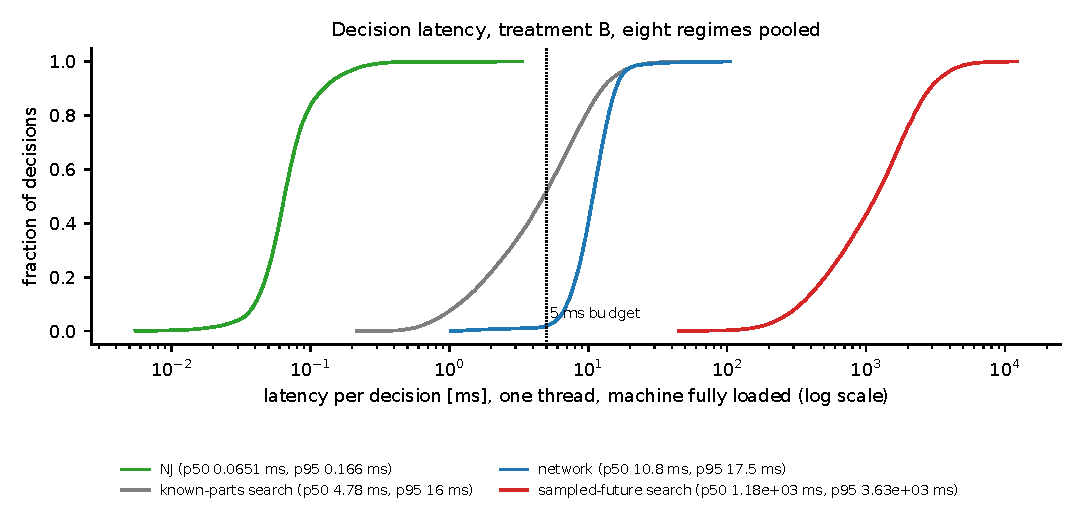
\includegraphics[width=\linewidth]{figures/latency.pdf}
\caption{Empirical distribution of the per-decision latency of the four policies on the
same decisions (basic mode, eight regimes pooled, one thread, machine fully loaded; log
scale). The dotted line is the 5~ms budget of the design.}
\label{fig:latency}
\end{figure}

\textbf{Design mode.} With pre-positioning allowed to every policy, the picture is the
same; the network's margin over \nj\ is smaller at the real load, because \nj\ itself
gains 7.4\,\% from pre-positioning there (Paper~2), and larger at the heavy load with
bursts. The network's level in the design mode against \nj\ in the basic mode, the
plan's original target, is $-14.1$\,\% on the real cell with Poisson arrivals (target:
at least $-10$\,\%).

%====================================================================
\section{Discussion}\label{sec:discussion}
%====================================================================

\subsection{What sets the quality of the policy}
Three facts of Section~\ref{sec:dev} point the same way. Networks of 0.88, 6.7 and 39
million parameters reach the same quality with the same teacher; every network reaches
its teacher within one or two iterations and then trades one validation group against
another; and changing the teacher moved the score by two points where changing the size
moved it by none. The quality of the amortized policy is the quality of the search that
labels its data, and the search's quality is set by what it scores (every part, not the
known ones), by how many futures it averages, and by not truncating. The learned value
head, which would make deeper or cheaper search possible, is the part that failed: its
error is set by the randomness of the future, which no decision changes, and that error
swamps the differences between candidates. A value that predicted the \emph{difference}
between candidates rather than the cost-to-go might do better; we did not try it.

\subsection{What the policy cannot do}
The confirmatory run shows two limits of the problem rather than of the method. At the
heavy load with a slow head, no policy beats the nearest-part rule by more than the noise:
with every belt queueing, the order in which the visible parts are served matters little
and the hidden queue, which none of the policies sees, is what would matter (Paper~2
measures it at 2.7--3.7\,\%). With bursts the gain of deciding better falls to 2\,\% on
the real cell, and a teacher that knows the burst model does not raise it: the
information that would help, whether the source is on now, is not in the state.

\subsection{Limits}\label{sec:limits}
The distance to the optimum is not measured. The project's exact models (a time-indexed
MILP and a CP-SAT model) support the makespan and the flow-time objectives but not the
penalized one, and a hindsight reference on the realized instances was deferred to a
second confirmatory run on new reserved realizations; the lower bounds of
Section~\ref{sec:properties} have been compared with offline solutions on small instances
only. The known-parts look-ahead is a rollout with $K=6$, not the exact search with
pruning that the project's plan foresaw; since its ceiling was found low before the exact
version was built, that search remains a verification tool for the known-parts
sub-problem rather than a method. The confirmatory regimes are eight variants of one
3-belt cell; the general cells with one to six conveyors appear only in the validation
of training, on development realizations. Latencies are for one CPU thread of a loaded
workstation and a 0.88~M-parameter model; a controller would run alone. Parts are points
with a minimum spacing, the head has no acceleration, processing times are constant in
the confirmatory regimes, and the penalty weights are placeholders. The reserved
realizations have been used once.

%====================================================================
\section{Conclusions}
%====================================================================
For a shared head over parallel conveyors whose belts stop for the head, the decision
that serves the parts in view best is not the best decision: a look-ahead that samples
the unknown arrivals and scores the realized cost of every part decides better than the
nearest-part rule by 3--8\,\% of the penalized flow time and than a look-ahead over the
known parts by 2--4 points, and a permutation-invariant pointer policy trained by expert
iteration on randomized cells reproduces that search within the noise at a hundredth of
its latency, 10~ms per decision on a loaded machine. The size of the network does not
matter beyond 0.88~M parameters; the teacher does. On reserved realizations of eight
regimes the policy beats the rule in seven and equals its teacher in all. What remains
open is how far all of this is from the optimum, which needs an exact reference for the
penalized objective and a new set of reserved realizations.

\bibliographystyle{plain}
\bibliography{../../literature/references}

\end{document}
